%%%%%%%%%%%%%%%%%%%% author.tex %%%%%%%%%%%%%%%%%%%%%%%%%%%%%%%%%%%
%
% sample root file for your "contribution" to a contributed volume
%
% Use this file as a template for your own input.
%
%%%%%%%%%%%%%%%% Springer %%%%%%%%%%%%%%%%%%%%%%%%%%%%%%%%%%%%%%%

%%%%%%%%%%%%%%%% Remove Warnings, KB#23 %%%%%%%%%%%%%%%%%%%%%%%%%
%\pdfminorversion=10
\RequirePackage{amsmath}
\RequirePackage{mathptmx}
% RECOMMENDED %%%%%%%%%%%%%%%%%%%%%%%%%%%%%%%%%%%%%%%%%%%%%%%%%%%
\documentclass[graybox]{svmult}

% choose options for [] as required from the list
% in the Reference Guide

\usepackage{graphicx, epstopdf}		%changed for windows, KB#23
\usepackage{newtxtext,newtxmath}
%\usepackage{mathptmx}       % selects Times Roman as basic font	%included before \documentclass, KB#23
\usepackage{helvet}         % selects Helvetica as sans-serif font  
\usepackage{courier}        % selects Courier as typewriter font
\usepackage{type1cm}        % activate if the above 3 fonts are
                            % not available on your system

\usepackage{makeidx}        % allows index generation

%\usepackage[dvips]{graphicx}		%commented for epstopdf for windows, KB#23
%\usepackage[dvipdfmx]{graphicx}
%\usepackage{graphicx}      % standard LaTeX graphics tool
                            % when including figure files
\usepackage{graphicx}
\usepackage{comment}
%\usepackage{subfig}
\usepackage{subfigure}
\usepackage{algorithmic}
\usepackage{algorithm}
\usepackage{cite}
%\usepackage{amsmath}		 %included before \documentclass, KB#23

\usepackage{multicol}        % used for the two-column index
\usepackage[bottom]{footmisc}% places footnotes at page bottom

\def\vector#1{\mbox{\boldmath $#1$}}



% see the list of further useful packages
% in the Reference Guide

\makeindex             % used for the subject index
                       % please use the style svind.ist with
                       % your makeindex program

%%%%%%%%%%%%%%%%%%%%%%%%%%%%%%%%%%%%%%%%%%%%%%%%%%%%%%%%%%%%%%%%%%%%%%%%%%%%%%%%%%%%%%%%%

\begin{document}

\title*{Research Report}

\subtitle{The Development of Haptic Feedback Data Glove for Enhancing Immersion in VR Experiences}
% Use \titlerunning{Short Title} for an abbreviated version of
% your contribution title if the original one is too long
\titlerunning{The Development of Haptic Feedback Data Glove for Enhancing Immersion in VR Experiences}
\author{Korntawat Witchuvanit}
\authorrunning{Korntawat Witchuvanit} 
% your contribution title if the original one is too long
\institute{
     Korntawat Witchuvanit
     \at Graduate School of Engineering, Fukuoka Institute of Technology (FIT), 3-30-1 Wajiro-Higashi, Higashi-Ku, Fukuoka 811--0295, Japan,
     \email{korntawat.contact@gmail.com}
     }


\maketitle

\abstract{In this research report, I will present my research for Master and PhD studies. First, I will introduce the present research, which is related with the application of Intelligent Algorithms (Fuzzy Logic) for admission control in 5G Wireless Networks considering Software Defined Networking (SDN) approach. Next, I will present my future research, which will be an Integrated Fuzzy-based System for Admission Control and Handover in 5G Wireless Networks. In order to deal with Base Station (BS) allocation in 5G, we will consider the application of Genetic Algorithms (GAs) and Particle Swarm Optimization (PSO). After that I will present the detailed plan for each year of my PhD studies. Finally, I will give the conclusions.}

\section{Introduction}
\label{sec:1}

	My Master studies at FIT is related with the application of Intelligent Algorithms (Fuzzy Logic) for admission control in 5G Wireless Networks considering Software Defined Networking (SDN) approach. The 5G network will be billions of new devices with unpredictable traffic pattern which provide high data rates. With the appearance of Internet of Things~(IoT), these devices will generate Big Data to the Internet, which will cause to congest and deteriorate the QoS \cite{8985528}. To resolve that problem, The 5G Wireless Network with reasonable admission control will help the network have good performance and great efficient management resource for the user to have a good experience in using the network.   
	
	In order to meet new network challenges and because traditional IP networks are complex and very hard to manage, network administrators have to identify and create new methodologies to enhance the network performance for the new era and SDN is one of them.  The SDN is a new networking paradigm that decouples the data plane from control plane in the network and promotes (logical) centralization of network control that have ability to program the network. Thus, the SDN can enhance system management efficiency and processing performance. As an example, the mobile handover mechanism with SDN can be used for reducing the delay in handover processing and improve the quality-of-service (QoS).
	
	A Fuzzy Logic (FL) system is a nonlinear mapping of an input data vector into a scalar output,  which is able to simultaneously handle numerical data and linguistic knowledge. The FL can deal with statements which may be true, false or intermediate truth-value.
	
	In my Master Thesis, I use FL to implement the proposed admission control system considering SDN.







%%%%%%%%%%%%%%%%%%%%%%%%%%%%%%%%%%%%%%%%%%%%%%%%%%%%%%%%%%%%%
%%%%%% Present Research
%%%%%%%%%%%%%%%%%%%%%%%%%%%%%%%%%%%%%%%%%%%%%%%%%%%%%%%%%%%%
\section{Present Research}\label{sec:Present Research}
\subsection{5G Wireless Networks Problems and Issues}
Recently, the growth of wireless technologies and user's demand of services are increasing rapidly. Especially in 5G networks, it will be billions of new devices with unpredictable traffic pattern which provide high data rates. With the appearance of Internet of Things~(IoT), these devices will generate Big Data to the Internet, which will cause to congest and deteriorate the QoS \cite{8985528}.

Compared to the 4G, the 5G, network is expect to be better than 4G. In Fig.~\ref{fig:4G5G} and Fig.~\ref{fig:5Gch} are shown the key challenges of 5G, which are improved  spectrum efficiency, reduced latency, low consumption, high data rate, capacity and throughput improvement. For example, the peak data for 5G is expected to be beyond 20 Gbps. In addition, the 5G network will provide users with new experiences such as Ultra High Definition Television (UHDT) on Internet and support a lot of IoT devices with long battery life and high data rates on hotspot areas with high user density.

 \begin{figure}[h!]\centering
	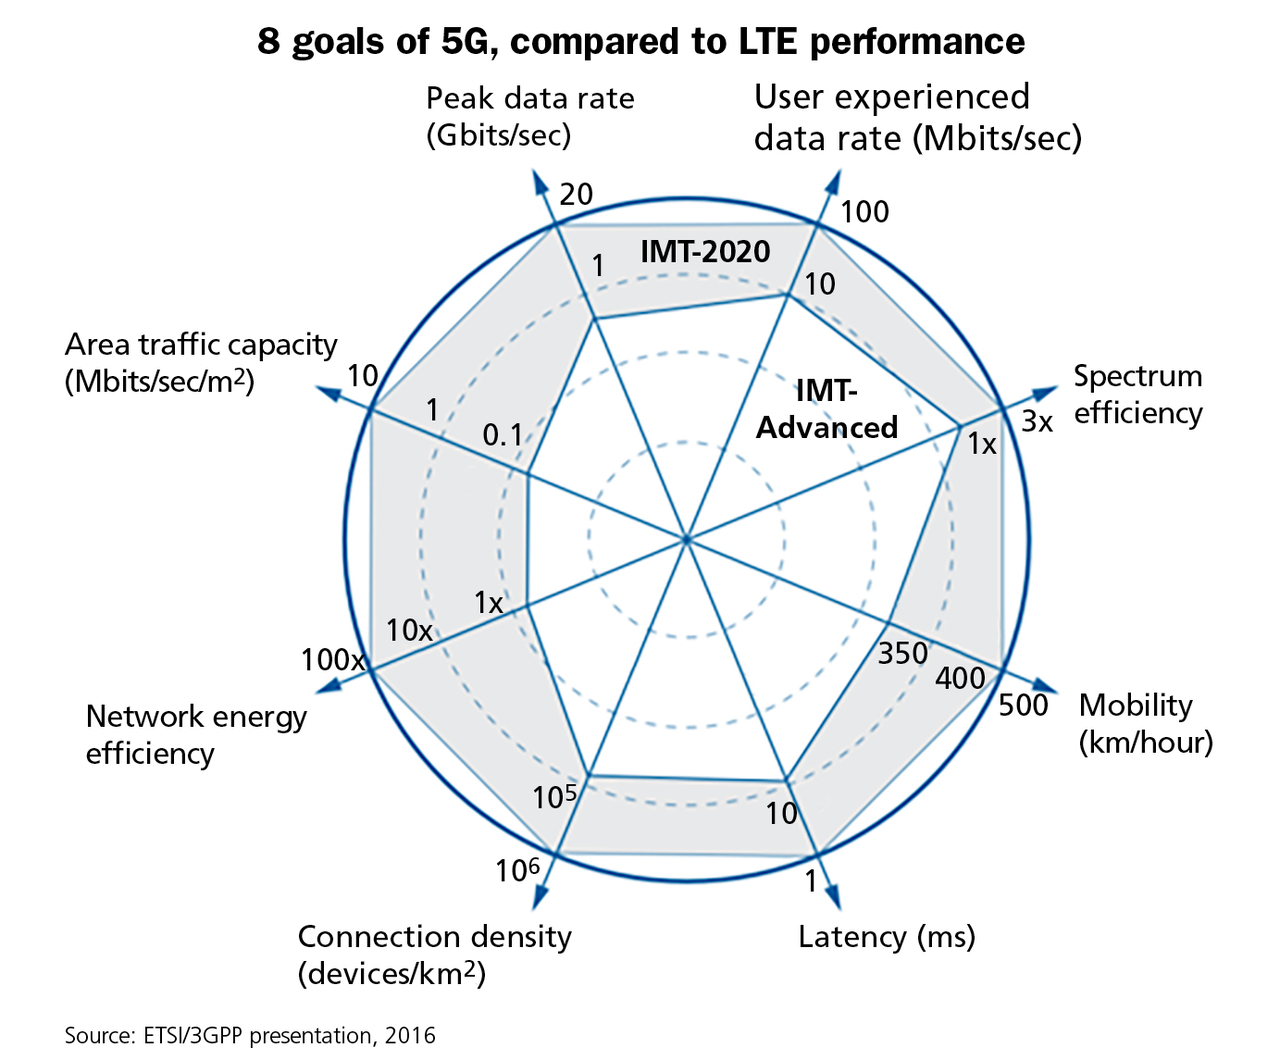
\includegraphics[width=0.6\textwidth]{figure/4G&5G.png}
	\caption{8 goals of 5G, compared to LTE performance.}\label{fig:4G5G}
\end{figure}
\begin{figure}[h!]\centering
	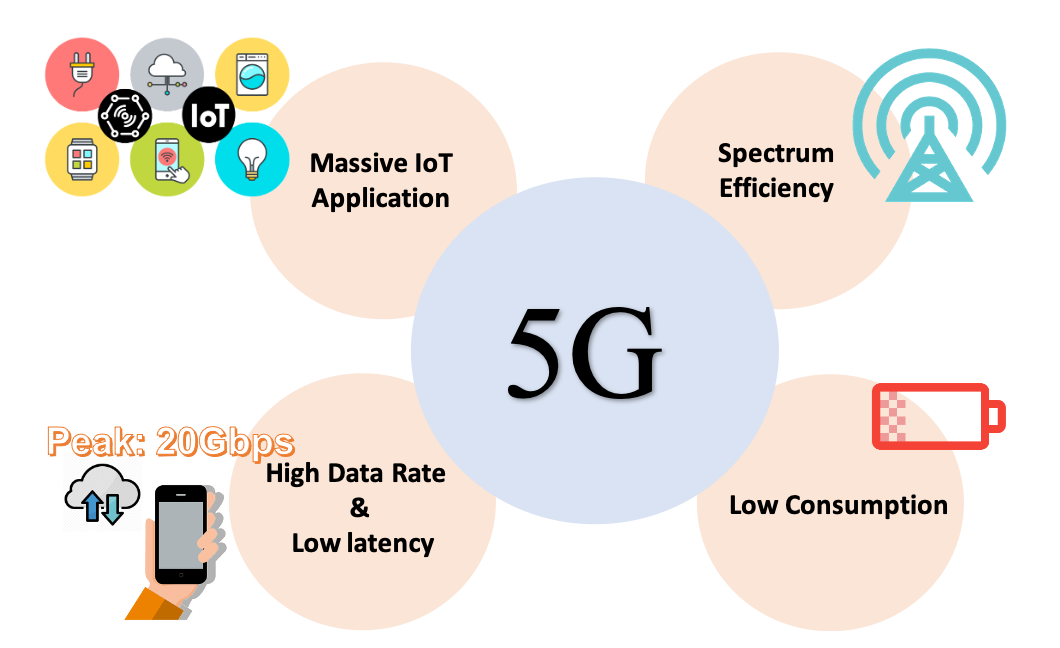
\includegraphics[width=0.85\textwidth]{figure/5G.eps}
	\caption{The key challenges of 5G.}\label{fig:5Gch}
\end{figure}


%%%%%%%%%%%%%%%%%%%%%%%%%%%%%%%%%%%%%%%%%%%%%%%%%%%%%%%%%%%%%
%%%%%% Software-Defined Networks (SDNs)
%%%%%%%%%%%%%%%%%%%%%%%%%%%%%%%%%%%%%%%%%%%%%%%%%%%%%%%%%%%%

\subsection{Software-Defined Networks (SDNs)}
\label{sec:sdn}
The SDN is  a new networking paradigm that decouples the data plane from control plane in the network. In traditional networks, the whole network is controlled by each network device. However, the traditional networks are hard to manage and control since they rely on physical infrastructure. Network devices must stay connected all the time when user wants to connect to other networks. Those processes must be based on the setting of each device, making controlling the operation of the network difficult. Therefore, they have to be set up one by one. In contrast, the SDN is easy to manage and provide network software based services from a centralised control plane. The SDN control plane is managed by SDN controller or cooperating group of SDN controllers. The SDN structure is shown in Fig.~\ref{fig:Structure of SDN}~\cite{6385040,mousa2016software}.
 
\begin{itemize}
\item \textbf{Application Layer} builds an abstracted view of the network by collecting information from the controller for decision-making purposes. The types of applications are  related to: network configuration and management, network monitoring, network troubleshooting, network policies and security.
\item \textbf{Control Layer} receives instructions or requirements from the Application Layer and control the Infrastructure Layer by using intelligent logic. 
\item \textbf{Infrastructure Layer} receives orders from SDN controller and sends data among them.
\end{itemize}

The SDN can manage network systems while enabling new services. In congestion traffic situation, management system can be flexible, allowing users to easily control and adapt  resources appropriately throughout the control plane. Mobility management is easier and quicker in forwarding across different wireless technologies (e.g.5G, 4G, Wifi and Wimax). Also, the handover procedure is simple and the delay can be decreased.

\begin{figure}[h]\centering
	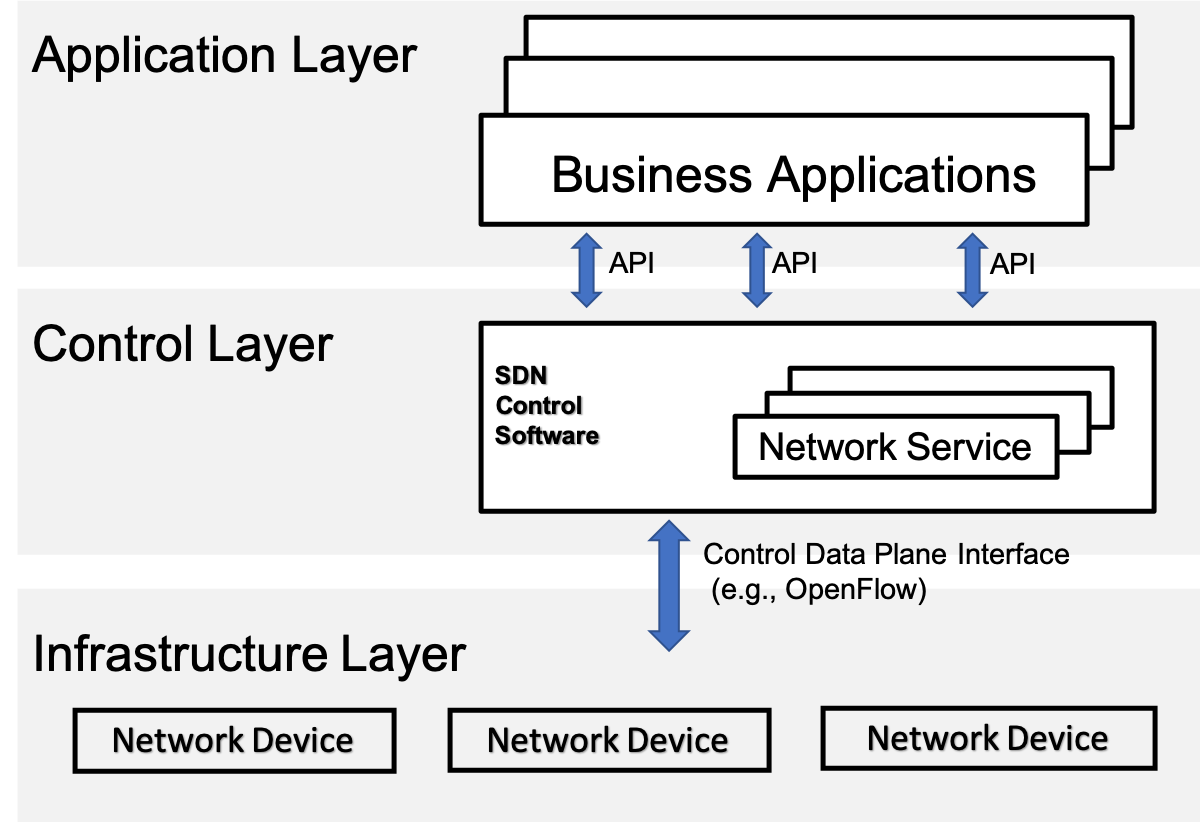
\includegraphics[width=0.8\textwidth]{figure/SDNs.png}
	\caption{Structure of SDN.}\label{fig:Structure of SDN}
\end{figure}



\subsection{Outline of Fuzzy Logic}\label{sec:fuzzy}
A Fuzzy Logic (FL) system is a nonlinear mapping of an input data vector into a scalar output,  which is able to simultaneously handle numerical data and linguistic knowledge. The FL can deal with statements which may be true, false or intermediate truth-value. These statements are impossible to quantify  using traditional mathematics. The FL system is used in many controlling applications such as aircraft control (Rockwell Corp.), Sendai subway operation (Hitachi), and TV picture adjustment (Sony).
 %add image and title
 
\begin{figure}[h]\centering
	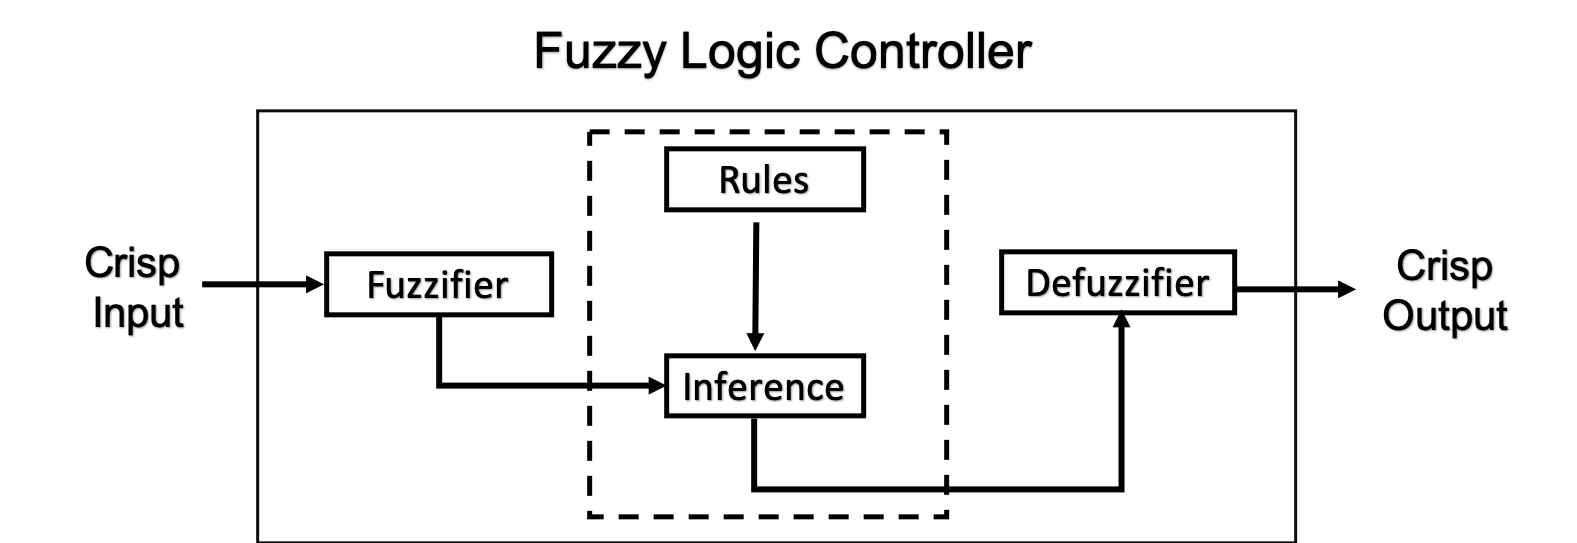
\includegraphics[width=1.0\textwidth]{figure/fc.png}%imagine location
	\caption{FLC structure.}\label{fig:Fuzzy Control System}%use name for ref.
\end{figure}

In Fig. \ref{fig:Fuzzy Control System} is shown Fuzzy Logic Controller (FLC) structure, which contains four components: fuzzifier, inference engine, fuzzy rule base and defuzzifier. 
\begin{itemize}
\item \textbf{Fuzzifier} is needed for combining the crisp values with rules which are linguistic variables and have fuzzy sets associated with them.
\item \textbf{The Rules} may be provided by expert or can be extracted from numerical data. In engineering case, the rules are expressed as a collection of IF-THEN statements. 
\item \textbf{The Inference Engine} infers fuzzy output by considering fuzzified input values and fuzzy rules.
\item \textbf{The Defuzzifier} maps output set into crisp numbers.
\end{itemize}




\subsubsection{Linguistic Variables}
A concept that plays a central role in 
the application of FL
is that of a linguistic variable. The linguistic variables 
may be viewed
as a form of data compression. One linguistic variable may represent many numerical variables. 
% We can classify the students of a class, by the score the got on the exam, 
% by only four linguistic variables: Bad, Passed, Good and Exellent, out of 100 numerical variables (points) in total.
It is suggestive to refer to this form of data compression as granulation.

The same effect can be achieved by conventional
quantization, but in the case of quantization,
the values are intervals, whereas in the case
of granulation the values are overlapping
fuzzy sets.
The advantages of granulation over quantization
are as follows:
\begin{itemize}
	\item it is more general;	
	\item it mimics the way in which humans interpret linguistic
	values;	
	\item the transition from one linguistic value to a contiguous
	linguistic value is gradual rather than abrupt,
	resulting in continuity and robustness.
\end{itemize}
For example, let Temperature (T) be interpreted as a linguistic variable. It can be decomposed into a set of Terms: T (Temperature) = \{Freezing, Cold, Warm, Hot, Blazing\}. Each term is characterised by fuzzy sets which can be interpreted, for instance, "Freezing" as a temparature below  $0^{\circ}C$, "Cold" as a temparature close to  $10^{\circ}C$.
 

\subsubsection{Fuzzy Control Rules}
Rules are usually written in the form "IF x is S THEN y is T" where x and y are linguistic variables that are expressed by  S and T, which are fuzzy sets. The x is a control (input) variable and y is the solution (output) variable. This rule is called Fuzzy control rule. The form "IF ... THEN" is called  a conditional sentence. It consists of "IF" which is called the antecedent and "THEN" is called the consequent. 
 

\subsubsection{Defuzzificaion Method}
There are many defuzzification methods, which are showing in following:
\begin{itemize}
 \item The Centroid Method; 
 \item Tsukamoto's Defuzzification Method;
 \item The Center of Are (COA) Method;
 \item The Mean of Maximum (MOM) Method;
 \item Defuzzification when Output of Rules are Function of Their Inputs.
\end{itemize}

%%%%%%%%%%%%%%%%%%%%%%%%%%%%%%%%%%%%%%%%%%%%%%%%%%%%%%%%%%%%%%%%%%%%%%%%%
%%%%%%%%%%%%%%%%%%%%%%%%%%%%%%%%%%%%%%%%%%%%%%%%%%%%%%%%%%%%%%%%%%%%%%%%%
% Proposed Fuzzy-based System
%%%%%%%%%%%%%%%%%%%%%%%%%%%%%%%%%%%%%%%%%%%%%%%%%%%%%%%%%%%%%%%%%%%%%%%%%
%%%%%%%%%%%%%%%%%%%%%%%%%%%%%%%%%%%%%%%%%%%%%%%%%%%%%%%%%%%%%%%%%%%%%%%%%
\subsection{Proposed Fuzzy-based System}\label{sec:proposed}
In this research, we use FL to implement the proposed system. In Fig.~\ref{fig:PSA}, we show the overview of our proposed approach. Each evolve Base Station (eBS) will receive controlling orders from SDN controller and they can communicate and send data with User Equipment (UE). On the other hand, the SDN controller will collect all the data about network traffic status and controlling eBS by using the proposed fuzzy-based approach. The SDN controller will be a communicating bridge between eBS and 5G core network.
%5gsdn
%\vspace{1cm}
\begin{figure}[h]\centering
	\includegraphics[width=0.8\textwidth]{figure/5gsdn.eps}
	\caption{Proposed system overview.}\label{fig:PSA}
\end{figure}
%\vspace{-1cm}
%\subsection{Proposed Fuzzy-based Simulation System}

The proposed system is called Integrated Fuzzy-based Admission Control System (IFACS) in 5G wireless networks. The structure of IFACS is shown in Fig.~\ref{fig:IFACS}. The IFACS system considers four input parameters: Quality of Service (QoS), Slice Priority (SP), User Request Delay Time (URDT) and Slice Overloading Cost (SOC). The output parameter is Admission Decision (AD)~\cite{AMPRIRIT2021100351}. For QoS, we use another Fuzzy-based system considering three parameters: Slice Throughput (ST), Slice Delay (SD) and Slice Loss (SL).

\begin{figure}[h]\centering
	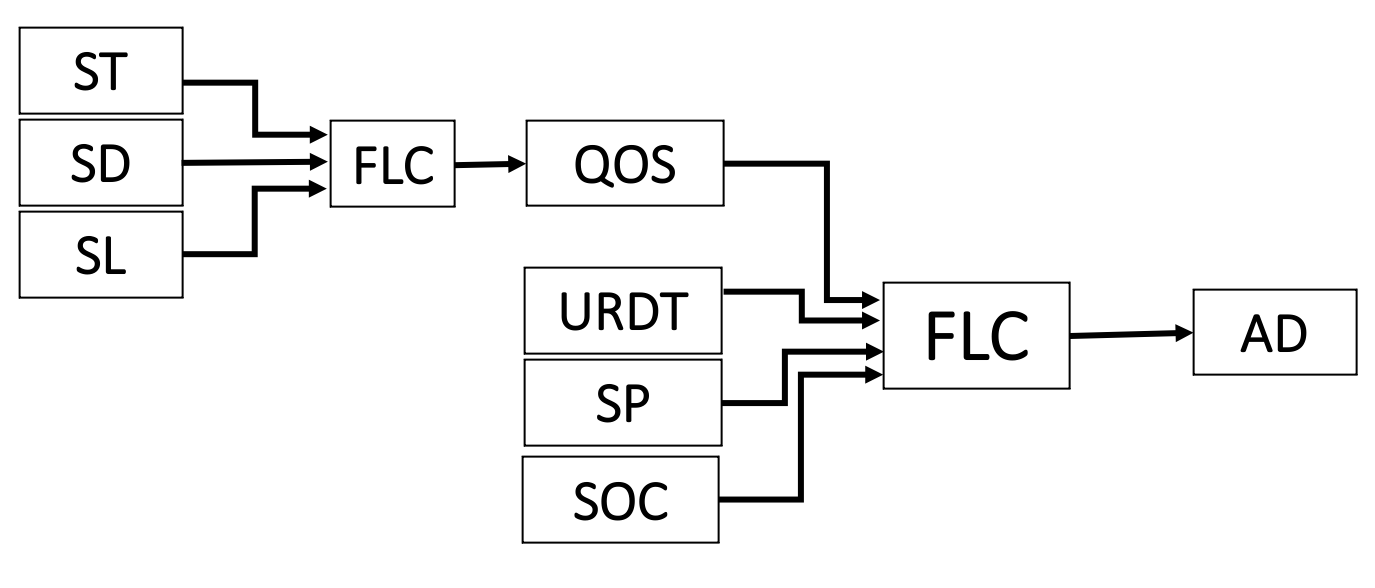
\includegraphics[width=0.85\textwidth]{figure/IFACS.eps}
	\caption{The structure of IFACS.}\label{fig:IFACS}
\end{figure}

\begin{figure}\centering
	\subfigure[SP=0.1]{
		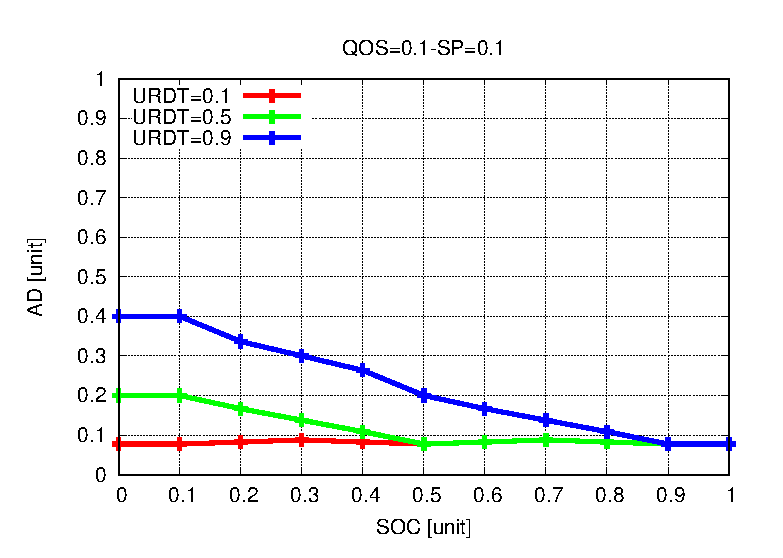
\includegraphics[width=0.48\textwidth]{figure/QOS=0.1-SP=0.1.eps}
		\label{subfig:RS21}
	}
	\subfigure[SP=0.5]{
		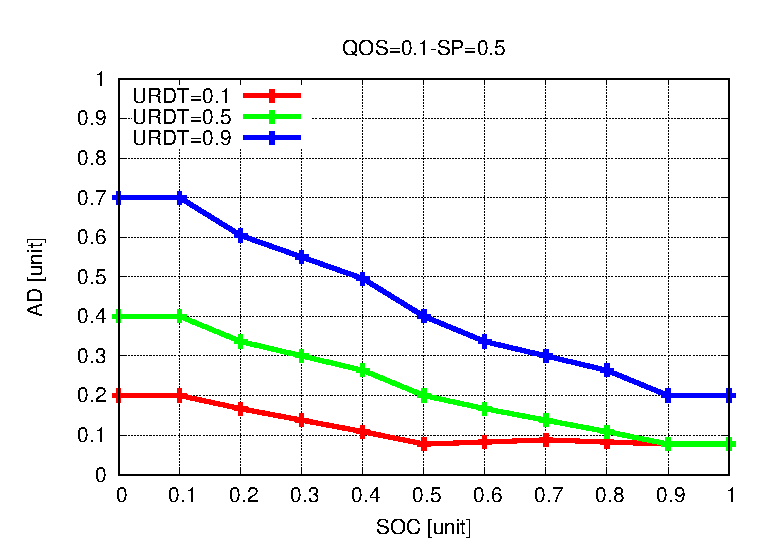
\includegraphics[width=0.48\textwidth]{figure/QOS=0.1-SP=0.5.eps}
		\label{subfig:RS22}
	}
	\subfigure[SP=0.9]{
		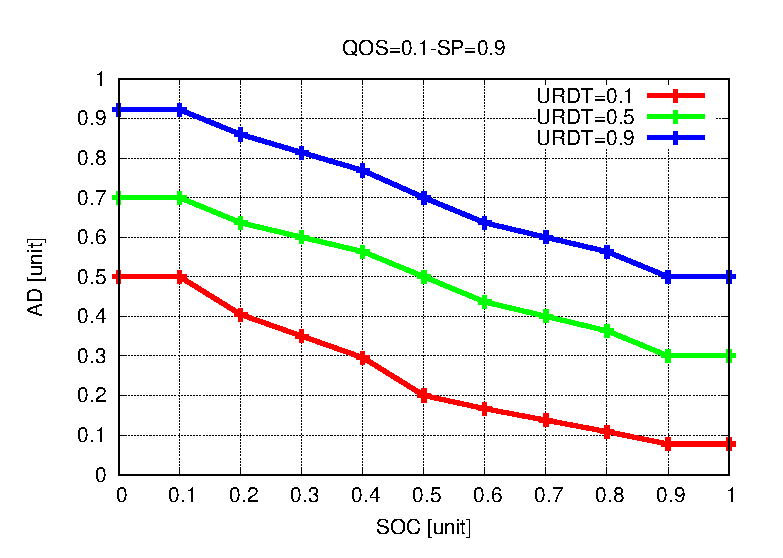
\includegraphics[width=0.48\textwidth]{figure/QOS=0.1-SP=0.9.eps}
		\label{subfig:RS23}
	}
	\caption{\label{fig:QOS0.1}Simulation results for IFACS (QoS=0.1).}
\end{figure}

\begin{figure}\centering
	\subfigure[SP=0.1]{
		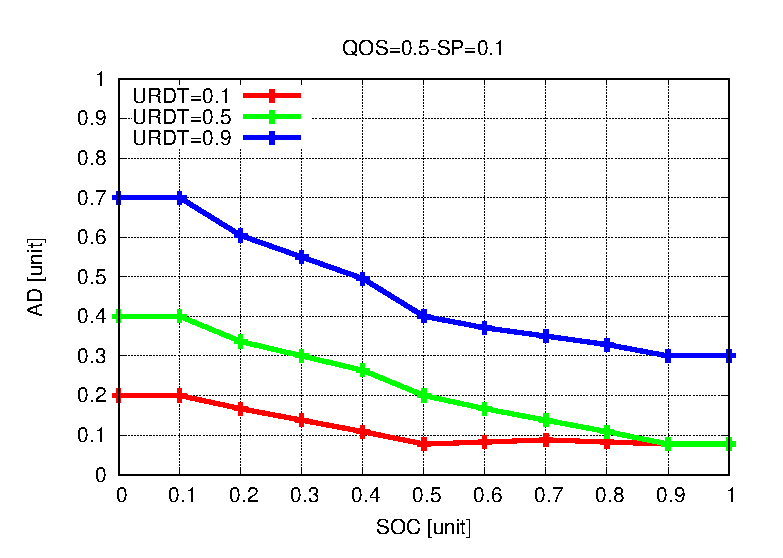
\includegraphics[width=0.48\textwidth]{figure/QOS=0.5-SP=0.1.eps}
		\label{subfig:RS27}
	}
	\subfigure[SP=0.5]{
		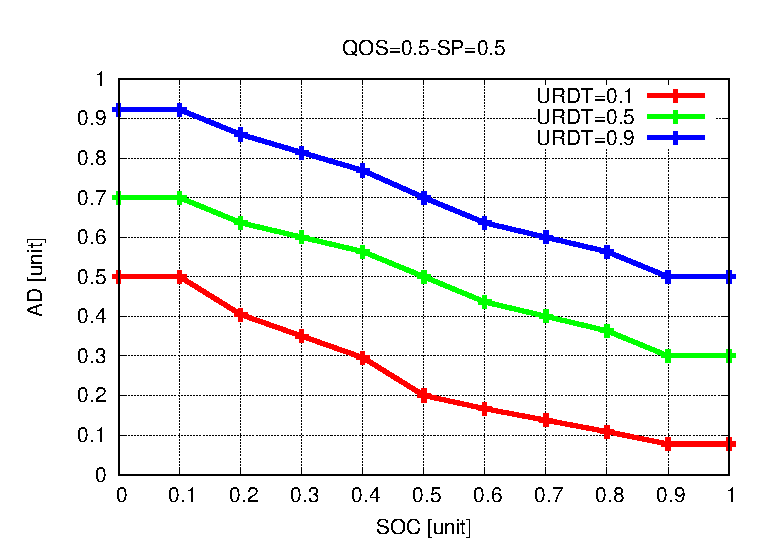
\includegraphics[width=0.48\textwidth]{figure/QOS=0.5-SP=0.5.eps}
		\label{subfig:RS28}
	}
	\subfigure[SP=0.9]{
		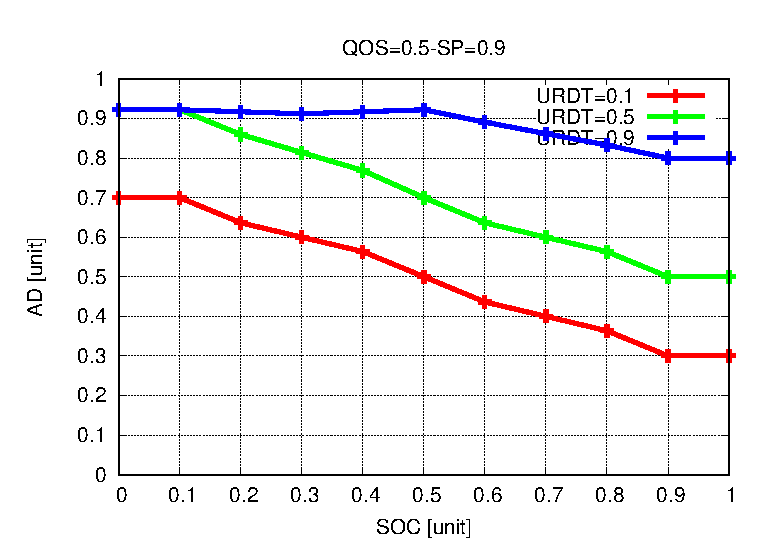
\includegraphics[width=0.48\textwidth]{figure/QOS=0.5-SP=0.9.eps}
		\label{subfig:SR29}
	}
	\caption{\label{fig:QOS0.5}Simulation results for IFACS (QoS=0.5).}
\end{figure}

\begin{figure}\centering
	\subfigure[SP=0.1]{
		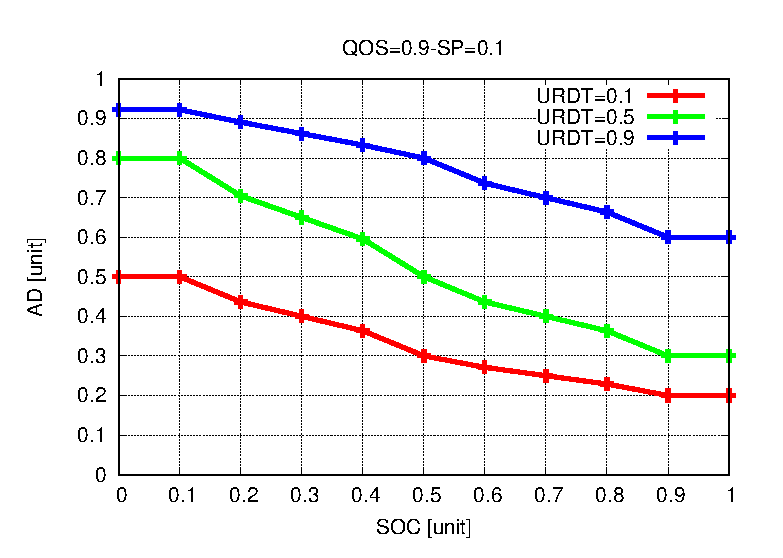
\includegraphics[width=0.48\textwidth]{figure/QOS=0.9-SP=0.1.eps}
		\label{subfig:RS213}
	}
	\subfigure[SP=0.5]{
		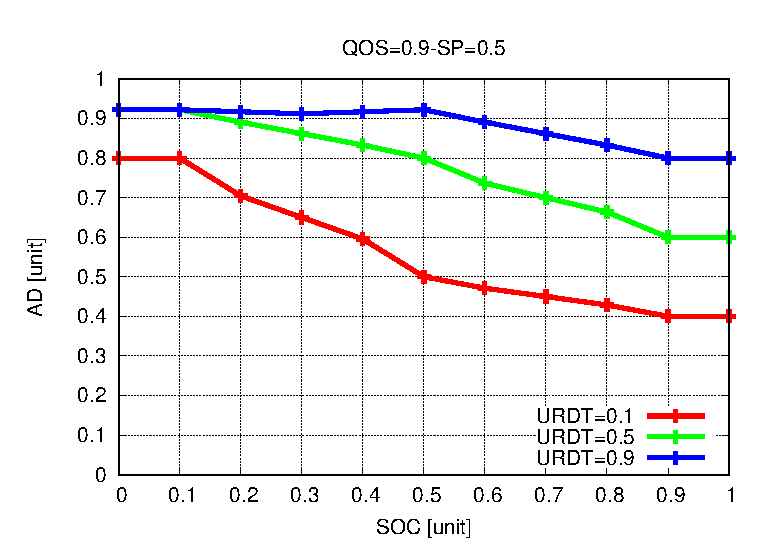
\includegraphics[width=0.48\textwidth]{figure/QOS=0.9-SP=0.5.eps}
		\label{subfig:RS214}
	}
	\subfigure[SP=0.9]{
		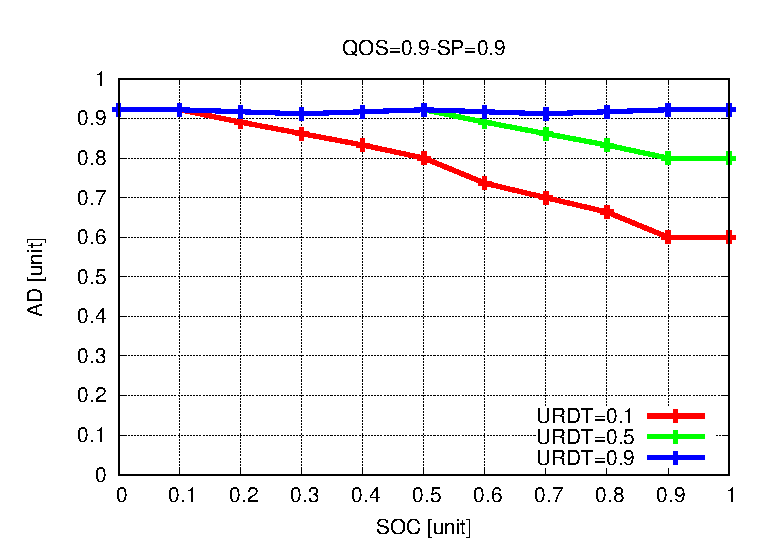
\includegraphics[width=0.48\textwidth]{figure/QOS=0.9-SP=0.9.eps}
		\label{subfig:SR215}
	}
	\caption{\label{fig:QOS0.9}Simulation results for IFACS (QoS=0.9).}
\end{figure}

The proposed system is evaluated by computer simulations. The simulation results are shown in Fig.~\ref{fig:QOS0.1}, Fig.~\ref{fig:QOS0.5} and Fig.~\ref{fig:QOS0.9}. They show the relation of AD with SOC. We consider URDT, QoS and SP as constant parameters. 

In Fig.~\ref{fig:QOS0.1}~(a), we consider the QoS value 0.1 and the SP value 0.1. When SOC is increased, we see that AD is decreased. For SOC 0.1, when URDT is increased from 0.1 to 0.5 and 0.5 to 0.9, the AD is increased by 12.25\% and 20\%, respectively. 

We compare Fig.~\ref{fig:QOS0.1}~(a) with Fig.~\ref{fig:QOS0.1}~(b) to see how SP has affected AD. We change the SP value from 0.1 to 0.9. The AD is increasing by 51.38\% when the SOC value is 0.3 and the URDT is 0.9. In Fig.~\ref{fig:QOS0.1}~(b), when we changed the SOC value from 0.3 to 0.7, the AD is decreased 20\% when the URDT value is 0.5. This is because a higher SOC value means the slice is more overloaded and the network can't provide the service for a new user.

In Fig.~\ref{fig:QOS0.5}, we increase the value of QoS to 0.5. The AD value in Fig.~\ref{fig:QOS0.5} is higher than in Fig.~\ref{fig:QOS0.1}. When the SP increases from 0.1 to 0.9, the AD increases 50\% when SOC value is 0.5 and the URDT value is 0.5. In Fig.~\ref{fig:QOS0.5}~(b), when URDT is 0.5, all AD values are higher than 0.5. This means that the system accepts all requests from new users.

In Fig.~\ref{fig:QOS0.9}, we increase the value of QoS to 0.9. We see that the AD value is increased much more compared with the results of Fig.~\ref{fig:QOS0.1} and Fig.~\ref{fig:QOS0.5}. 


From the simulations results, we conclude as when QoS, SP and URDT value are increased, the AD value is increased. But, when the SOC parameter is increased, the AD value is decreased.


%\vspace{1000mm}
\section{PhD Research}

My PhD studies will be related with improving the Integrated Fuzzy-based Admission Control System  (IFACS) and the integration of IFACS and handover for 5G wireless networks. In following, I will present 5G Handover, Genetic Algorithms (GAs) and Particle Swarm Optimization (PSO).

%The 5G handover problems
The future network will provide better coverage, high capacity, low latency and highly reliable connectivity. The handover is an important process to select the next cell that the user should be connected. If handover failure happen, the User Equipment (UE) will fail to connect to the next cell. In 5G, a  massive number of small 5G Base Stations (BS)  using higher mm-wave bands will make the coverage smaller. This will lead to a high number of handovers which interrupt the call and degradate the throughput. For resolving this problem and providing seamless service to the user, an efficient method is needed to improve the handover procedure. 


%Genetic Algorithms
The GAs are Evolution Computation (EC) techniques which search for optimal solution to a problem. These algorithms encode a potential solution to a specific problem on a simple chromosome-like data structure and apply recombination operators to these structures to preserve critical information. In every generation, a new set of chromosome is recreated  using parts of the fittest members from the old set. When the results become the target goal, the process will be finished. These algorithms evolve the generation using following operators: Selection Operator, Crossover Operator, Mutation Operator. GAs are often viewed as function optimizer which generate high-quality solution for optimization problem and search. 

%Particle swarm optimization
PSO is a swarm intelligence based numerical optimization algorithm inspired from birds’ flocking or fish schooling for the solution of nonlinear, nonconvex or combinatorial optimization problems
\cite{bansal2019evolutionary}. In PSO, the solution is obtained by a random search which is done by a set of randomly generated potential solutions. Each potential solution is called a particle and the collection of potential solutions is called a swarm. The particle will move to the search domain for searching optimal solution by a specified velocity and keeps the track of its previous best position. Comparing with its previous best position, it will choose the best position for the solution. PSO has been applied to solve a variety of optimization problems and its performance is
compared with other popular stochastic search techniques like Genetic algorithms, Differential Evolution, Simulated Annealing and so on \cite{Pant2009}. 

\begin{figure}[h]\centering
	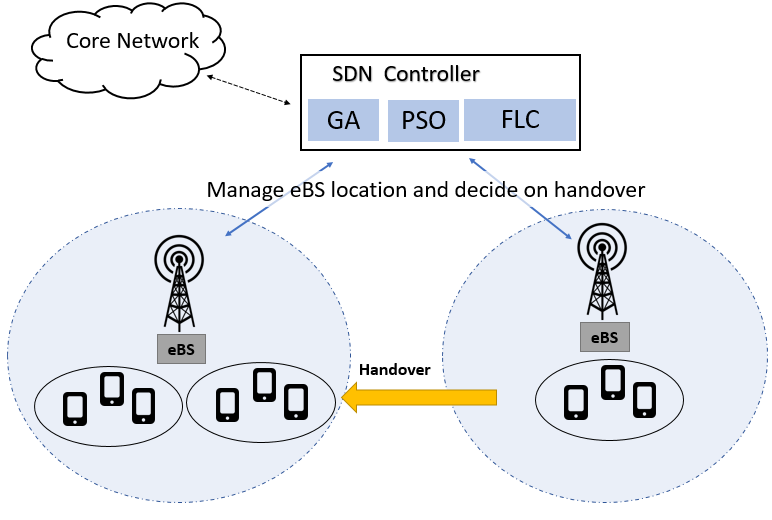
\includegraphics[width=0.7\textwidth]{figure/GAhandover.png}
	\caption{Proposed system overview.}\label{fig:PShand}
\end{figure}

In Fig.~\ref{fig:PShand}, we show the overview of our proposed approach. The SDN controller will calculate the best location of eBSs in order to have better coverage area for user by using GA and PSO. When a user can not be accepted to present eBS, then it will be handovered to the neighbor eBS. This handover will be considered as a new call admission control in neighbor eBS.

%When the eBS is the best location for connecting to user and handover, the SDN controller will collect all the data about network traffic status and controlling eBS for making decision on handover by using the proposed fuzzy-based approach.

By utilizing SDN technology, the Network Slicing is proposed to enable full implementation of a diversity 5G application scenarios. The proposed system will consider various 5G scenarios and make the best decision for 5G handover.	

Moreover, I will consider other parameters and make extensive simulations to evaluate IFACS for admission control.




\section{Future Work and Annual Research Plan}
\label{sec:conc}
My PhD research plan includes the following topics:
\begin{itemize}
	\item Proposal of new parameters for IFACS.
	\item Experiments with IFACS. 
	\item Comparison of simulation results with other systems and research works.
	\item Comparison of simulation results with experimented results.
\end{itemize}

The detailed plan for each year is as follows.
\begin{enumerate}
	\item In the first year, I will deal with following issues.
	\begin{itemize}
		\item Proposal of new parameters for IFACS
		\item Proposal of new parameters for QoS Evaluation.
		\item Implementation of proposed systems. 
		\item Evaluation of proposed systems.
	\end{itemize}
	\item In the second year, I will deal with following issues.
	\begin{itemize}
		\item Experiments with IFACS. 
		\item Comparison between simulation results and experiment result.
		\item Comparison with other research works.
	\end{itemize}
	\item In the last year, I will deal with the following issues.
	\begin{itemize}
		\item Implementation of integrated call admission control and handover for 5G wireless networks.
		\item Writing of PhD Thesis.
	\end{itemize}
\end{enumerate}


\section{Conclusions}
In this report, I presented my research during Master studies. Then, I introduced 5G Wireless Networks, SDN, FL, GAs and PSO as related technologies and approaches for my PhD studies.


\bibliographystyle{ieeetr}
\bibliography{ref}


\end{document}
